\subsection{\textbf{Sprint 3}}

No início desta \textit{sprint}, tomamos a decisão estratégica de focar em um único mapa, mais complexo que a versão inicial, mas ainda relativamente simples para garantir o progresso contínuo do projeto. Imediatamente percebi uma melhora significativa na comunicação dos \ac{ages} IV, bem como na qualidade das descrições das tarefas no quadro, o que facilitou consideravelmente o alinhamento entre as expectativas e as implementações necessárias.

Durante a primeira aula, realizamos uma sessão de \textit{brainstorming} para definir a implementação da funcionalidade de popular o banco de dados, determinando também o formato adequado do arquivo CSV esperado pelo \textit{endpoint}. Após discussões produtivas, chegamos a uma solução elegante e funcional: o CSV deveria conter uma linha para cada produto, simplificando o processo de importação e manutenção dos dados.

Minha responsabilidade principal nesta \textit{sprint} foi desenvolver uma segunda versão do mapa, incluindo mais estandes e um indicador visual da localização do totem. Graças ao estudo aprofundado que havia realizado sobre a biblioteca Three.js \cite{threejs}, consegui criar rapidamente uma versão aprimorada que atendeu às expectativas como protótipo funcional.

\begin{figure}[H]
    \centering
    \small
    \caption{Mapa desenvolvido}
    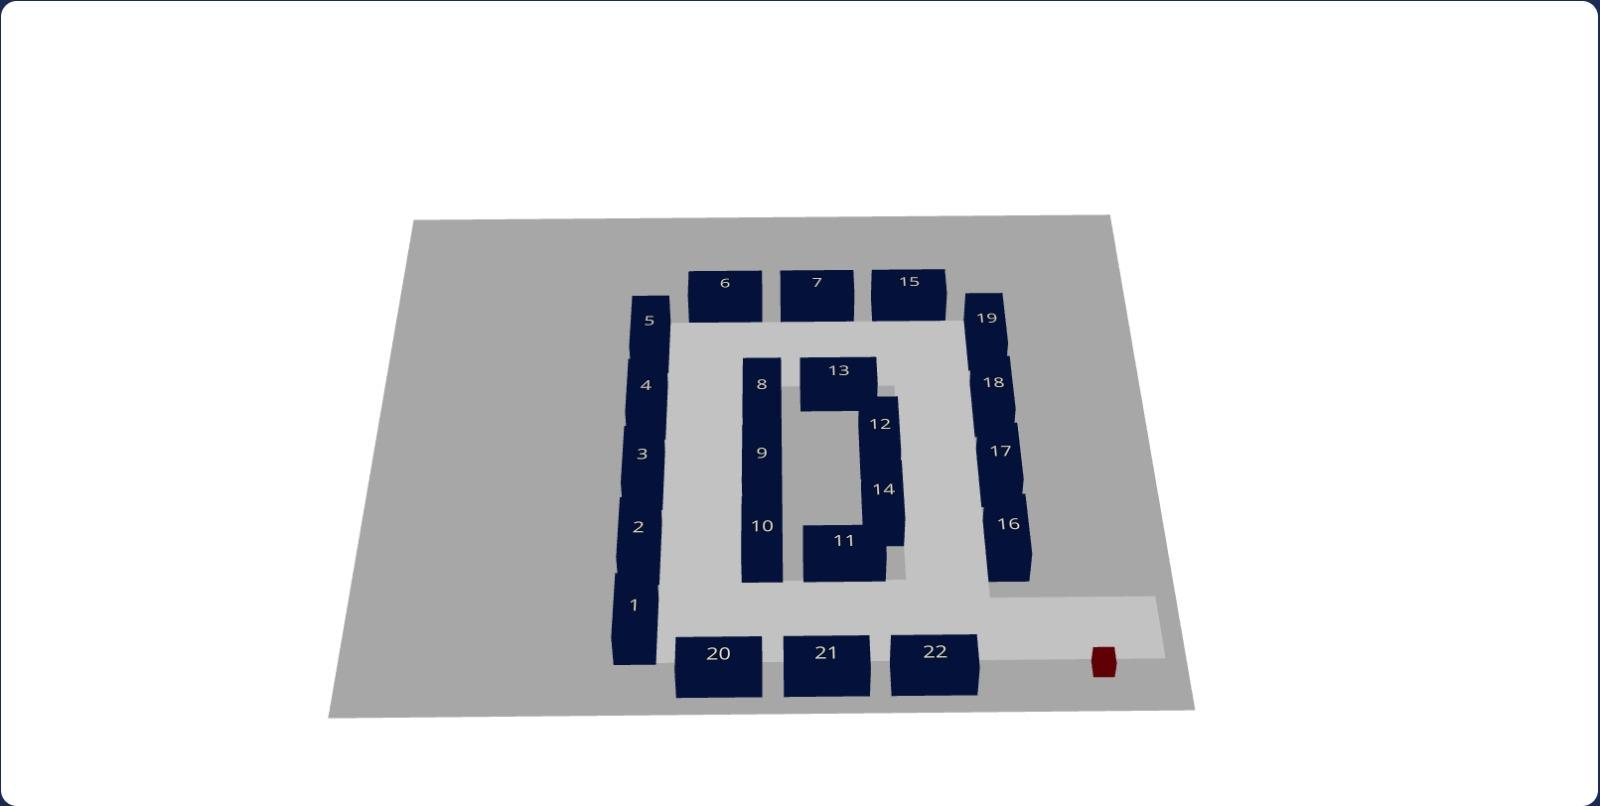
\includegraphics[width=0.9\linewidth]{conteudo/4 - ages III/images/fig8-mapa-desenvolvido.jpg}

    Fonte: Código \textit{frontend} do projeto \cite{wikiTotem}
    \label{fig:totem-mapa-desenvolvido}
\end{figure}

Com o mapa desenvolvido, direcionei meus esforços para realizar a integração com o \textit{backend}. Surpreendentemente, a tarefa foi menos complexa do que havia antecipado, pois o repositório do \textit{frontend} já estava adequadamente estruturado para suportar a integração. Foram necessárias apenas algumas modificações pontuais para garantir uma integração completa e funcional.

Concluída minha implementação principal, voltei a apoiar o desenvolvimento do \textit{backend} junto aos \ac{ages} II. Os dois responsáveis pela funcionalidade de popular o banco estavam com bom progresso, enquanto a terceira \ac{ages} II aperfeiçoava a estrutura do \textit{backend}, incluindo a documentação Swagger \cite{swagger} nos \textit{controllers}, trabalho que também estava bem encaminhado.

Durante uma aula, em conjunto com os \ac{ages} IV, decidimos explorar uma abordagem inovadora para o mapa. O \textit{stakeholder} havia mencionado no início do semestre sua visão de utilizar o sistema no Tecnopuc, onde a multiplicidade de prédios e empresas torna desafiadora a localização para visitantes externos. Motivados por essa ideia e buscando compensar a entrega insatisfatória da \textit{sprint} anterior, decidimos replicar o mapa do Tecnopuc como uma funcionalidade surpresa.

Aplicando o conhecimento adquirido, consegui implementar o mapa do Tecnopuc sem grandes dificuldades, obtendo aprovação imediata dos \ac{ages} IV quanto à qualidade e fidelidade da representação.

\begin{figure}[H]
    \centering
    \small
    \caption{Primeira versão do mapa do Tecnopuc}
    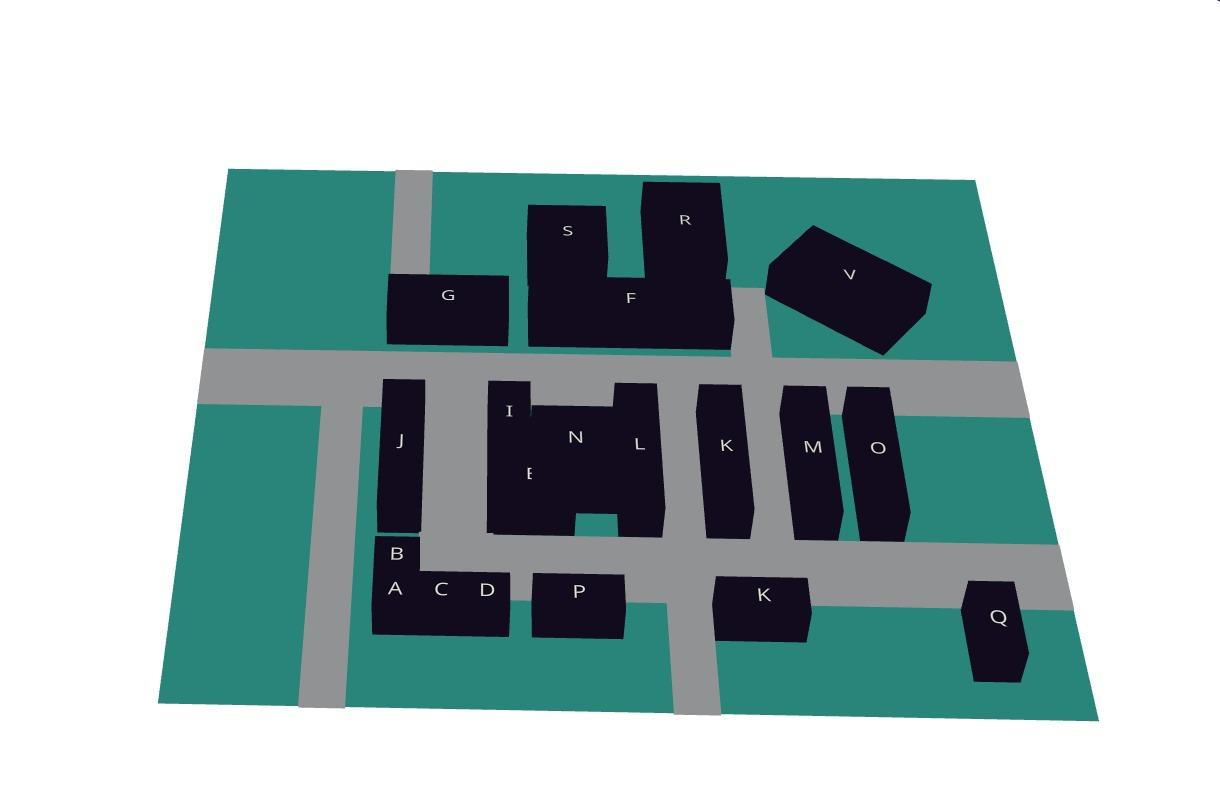
\includegraphics[width=0.9\linewidth]{conteudo/4 - ages III/images/fig9-mapa-tecnopuc-v1.jpg}

    Fonte: Repositório \textit{frontend} do projeto \cite{wikiTotem}
    \label{fig:totem-tecnopuc-v1}
\end{figure}

Com minhas tarefas concluídas, dediquei-me à revisão dos \textit{pull requests} dos \ac{ages} II durante a fase de \textit{code freeze}. Não identificamos problemas significativos no código do \textit{backend}. Contudo, uma funcionalidade delegada a outro \ac{ages} III e um \ac{ages} I não foi finalizada, resultando em débito técnico --- felizmente, algo que passaria despercebido aos olhos do \textit{stakeholder}.

Durante a última semana e meia da \textit{sprint}, enfrentamos sérios problemas com o ambiente GitLab, incluindo indisponibilidade, lentidão extrema e um \textit{rollback} crítico poucos dias antes do \textit{code freeze}. Embora o projeto não tenha sido severamente afetado, a situação gerou apreensão na equipe sobre possíveis recorrências.

A apresentação desta \textit{sprint} foi um sucesso completo, contrastando drasticamente com a anterior. O \textit{stakeholder} demonstrou extrema satisfação com o progresso, afirmando que apenas com o desenvolvimento realizado até aquele momento, a ideia do projeto já estava validada. Estrategicamente, não havíamos revelado o desenvolvimento do mapa do Tecnopuc. Quando o \textit{stakeholder} sugeriu focar a última \textit{sprint} em um caso de uso específico para o Tecnopuc, os \ac{ages} IV apresentaram nossa implementação surpresa. Sua reação foi de genuíno contentamento, prontificando-se imediatamente a fornecer qualquer informação adicional necessária sobre o local.

Esta \textit{sprint} representou um ponto de virada no projeto, não apenas pelos avanços técnicos significativos, mas também pela validação do conceito pelo \textit{stakeholder} e pelo restabelecimento da confiança na capacidade de entrega da equipe.

É importante destacar que, durante esta \textit{sprint}, o \ac{ages} III Eduardo Felber Eichner e eu acabamos assumindo responsabilidades adicionais para garantir a continuidade do projeto. Estabelecemos uma divisão clara de trabalho, onde Eduardo concentrou-se exclusivamente no repositório \textit{frontend} enquanto eu gerenciava o \textit{backend} e desenvolvia os mapas. Embora essa abordagem tenha sido eficaz e garantido o sucesso das entregas, reconheço que deveria ter comunicado mais claramente minhas preocupações sobre a distribuição desigual de responsabilidades entre todos os \ac{ages} III.
